% Options for packages loaded elsewhere
\PassOptionsToPackage{unicode}{hyperref}
\PassOptionsToPackage{hyphens}{url}
\PassOptionsToPackage{dvipsnames,svgnames,x11names}{xcolor}
%
\documentclass[
  letterpaper,
  DIV=11,
  numbers=noendperiod]{scrartcl}

\usepackage{amsmath,amssymb}
\usepackage{iftex}
\ifPDFTeX
  \usepackage[T1]{fontenc}
  \usepackage[utf8]{inputenc}
  \usepackage{textcomp} % provide euro and other symbols
\else % if luatex or xetex
  \usepackage{unicode-math}
  \defaultfontfeatures{Scale=MatchLowercase}
  \defaultfontfeatures[\rmfamily]{Ligatures=TeX,Scale=1}
\fi
\usepackage{lmodern}
\ifPDFTeX\else  
    % xetex/luatex font selection
\fi
% Use upquote if available, for straight quotes in verbatim environments
\IfFileExists{upquote.sty}{\usepackage{upquote}}{}
\IfFileExists{microtype.sty}{% use microtype if available
  \usepackage[]{microtype}
  \UseMicrotypeSet[protrusion]{basicmath} % disable protrusion for tt fonts
}{}
\makeatletter
\@ifundefined{KOMAClassName}{% if non-KOMA class
  \IfFileExists{parskip.sty}{%
    \usepackage{parskip}
  }{% else
    \setlength{\parindent}{0pt}
    \setlength{\parskip}{6pt plus 2pt minus 1pt}}
}{% if KOMA class
  \KOMAoptions{parskip=half}}
\makeatother
\usepackage{xcolor}
\setlength{\emergencystretch}{3em} % prevent overfull lines
\setcounter{secnumdepth}{-\maxdimen} % remove section numbering
% Make \paragraph and \subparagraph free-standing
\ifx\paragraph\undefined\else
  \let\oldparagraph\paragraph
  \renewcommand{\paragraph}[1]{\oldparagraph{#1}\mbox{}}
\fi
\ifx\subparagraph\undefined\else
  \let\oldsubparagraph\subparagraph
  \renewcommand{\subparagraph}[1]{\oldsubparagraph{#1}\mbox{}}
\fi


\providecommand{\tightlist}{%
  \setlength{\itemsep}{0pt}\setlength{\parskip}{0pt}}\usepackage{longtable,booktabs,array}
\usepackage{calc} % for calculating minipage widths
% Correct order of tables after \paragraph or \subparagraph
\usepackage{etoolbox}
\makeatletter
\patchcmd\longtable{\par}{\if@noskipsec\mbox{}\fi\par}{}{}
\makeatother
% Allow footnotes in longtable head/foot
\IfFileExists{footnotehyper.sty}{\usepackage{footnotehyper}}{\usepackage{footnote}}
\makesavenoteenv{longtable}
\usepackage{graphicx}
\makeatletter
\def\maxwidth{\ifdim\Gin@nat@width>\linewidth\linewidth\else\Gin@nat@width\fi}
\def\maxheight{\ifdim\Gin@nat@height>\textheight\textheight\else\Gin@nat@height\fi}
\makeatother
% Scale images if necessary, so that they will not overflow the page
% margins by default, and it is still possible to overwrite the defaults
% using explicit options in \includegraphics[width, height, ...]{}
\setkeys{Gin}{width=\maxwidth,height=\maxheight,keepaspectratio}
% Set default figure placement to htbp
\makeatletter
\def\fps@figure{htbp}
\makeatother
% definitions for citeproc citations
\NewDocumentCommand\citeproctext{}{}
\NewDocumentCommand\citeproc{mm}{%
  \begingroup\def\citeproctext{#2}\cite{#1}\endgroup}
\makeatletter
 % allow citations to break across lines
 \let\@cite@ofmt\@firstofone
 % avoid brackets around text for \cite:
 \def\@biblabel#1{}
 \def\@cite#1#2{{#1\if@tempswa , #2\fi}}
\makeatother
\newlength{\cslhangindent}
\setlength{\cslhangindent}{1.5em}
\newlength{\csllabelwidth}
\setlength{\csllabelwidth}{3em}
\newenvironment{CSLReferences}[2] % #1 hanging-indent, #2 entry-spacing
 {\begin{list}{}{%
  \setlength{\itemindent}{0pt}
  \setlength{\leftmargin}{0pt}
  \setlength{\parsep}{0pt}
  % turn on hanging indent if param 1 is 1
  \ifodd #1
   \setlength{\leftmargin}{\cslhangindent}
   \setlength{\itemindent}{-1\cslhangindent}
  \fi
  % set entry spacing
  \setlength{\itemsep}{#2\baselineskip}}}
 {\end{list}}
\usepackage{calc}
\newcommand{\CSLBlock}[1]{\hfill\break\parbox[t]{\linewidth}{\strut\ignorespaces#1\strut}}
\newcommand{\CSLLeftMargin}[1]{\parbox[t]{\csllabelwidth}{\strut#1\strut}}
\newcommand{\CSLRightInline}[1]{\parbox[t]{\linewidth - \csllabelwidth}{\strut#1\strut}}
\newcommand{\CSLIndent}[1]{\hspace{\cslhangindent}#1}

\usepackage{booktabs}
\usepackage{caption}
\usepackage{longtable}
\usepackage{colortbl}
\usepackage{array}
\KOMAoption{captions}{tableheading}
\makeatletter
\@ifpackageloaded{caption}{}{\usepackage{caption}}
\AtBeginDocument{%
\ifdefined\contentsname
  \renewcommand*\contentsname{Table of contents}
\else
  \newcommand\contentsname{Table of contents}
\fi
\ifdefined\listfigurename
  \renewcommand*\listfigurename{List of Figures}
\else
  \newcommand\listfigurename{List of Figures}
\fi
\ifdefined\listtablename
  \renewcommand*\listtablename{List of Tables}
\else
  \newcommand\listtablename{List of Tables}
\fi
\ifdefined\figurename
  \renewcommand*\figurename{Figure}
\else
  \newcommand\figurename{Figure}
\fi
\ifdefined\tablename
  \renewcommand*\tablename{Table}
\else
  \newcommand\tablename{Table}
\fi
}
\@ifpackageloaded{float}{}{\usepackage{float}}
\floatstyle{ruled}
\@ifundefined{c@chapter}{\newfloat{codelisting}{h}{lop}}{\newfloat{codelisting}{h}{lop}[chapter]}
\floatname{codelisting}{Listing}
\newcommand*\listoflistings{\listof{codelisting}{List of Listings}}
\makeatother
\makeatletter
\makeatother
\makeatletter
\@ifpackageloaded{caption}{}{\usepackage{caption}}
\@ifpackageloaded{subcaption}{}{\usepackage{subcaption}}
\makeatother
\ifLuaTeX
  \usepackage{selnolig}  % disable illegal ligatures
\fi
\usepackage{bookmark}

\IfFileExists{xurl.sty}{\usepackage{xurl}}{} % add URL line breaks if available
\urlstyle{same} % disable monospaced font for URLs
\hypersetup{
  pdftitle={Physical activity as an effect modificator of lifestyle factors on small vessel deisease burden},
  colorlinks=true,
  linkcolor={blue},
  filecolor={Maroon},
  citecolor={Blue},
  urlcolor={Blue},
  pdfcreator={LaTeX via pandoc}}

\title{Physical activity as an effect modificator of lifestyle factors
on small vessel deisease burden}
\author{Andreas Gammelgaard Damsbo \and Rolf Ankerlund
Blauenfeldt \and Sigrid Breinholt Vestergaard \and Niels Lech
Pedersen \and Kim Morgenstjerne Østerskov \and Mette Foldager
Hindsholm \and Arzu Bilgin-Freiert \and Claus Ziegler
Simonsen \and Rikke Beese Dalby \and Grethe Andersen \and Janne
Kaergaard Mortensen}
\date{}

\begin{document}
\maketitle
\begin{abstract}
\textbf{Background and aims} Physical activity (PA) may reduce the
development of small vessel disease (SVD). The effect of physical
activity and more classical vascular risk factors such as hypertension
and diabetes in the development of SVD is debated, however. We aim to
investigate the effect modification of physical activity on traditional
vascular risk factors and the burden of small vessel disease among acute
ischemic stroke patients.

\textbf{Methods} We have pooled patients from two clinical trials on
acute ischemic stroke treatment. The main outcome is an ordinal scale
score of quantified MR biomarkers of small vessel disease (SVD) burden
based on visually assessed acute stroke scans (T2* or SWI and FLAIR
sequences). Biomarkers includes microbleeds, old lacunar infarcts,
superficial siderosis, white matter hyperintensities and atrophy.
Covariates includes age, sex, pre-stroke physical activity, diabetes,
hypertension, atrial fibrillation and previous cardiovascular diseases.
Pre-stroke PA was assessed with a questionnaire on inclusion within a
few days after stroke onset. Data will be analyzed using bivariate and
multivariate linear regression analysis.

\textbf{Results} We expect to include a total of around 1000 adult
patients admitted to the comprehensive stroke centre at Aarhus
University Hospital between 2013-2022. Preliminary results will be
presented at ESOC 2024.

\textbf{Conclusions} Physical activity may be an important factor in
modifying the risk of SVD development in stroke patients.
\end{abstract}

\textsubscript{Source:
\href{https://agdamsbo.github.io/svd-modification/index.qmd.html}{Article
Notebook}}

\subsection{Introduction}\label{introduction}

THe correlation between physical activity, small vessel disease and
classical risk factors is very much debated and not fully
understood.(Moniruzzaman et al. 2020; Torres et al. 2019; Landman et al.
2021)

In this abstract, we present the preliminary results from our pooled SVD
study, also presented at
\href{https://apps.congrex.com/esoc2024/en-GB/pag/presentation/362937}{ESOC
2024}.

\subsection{Methods}\label{methods}

This study is a cross-sectional study, based on a pooled dataset from
two different randomised, clinical trials on patients with acute stroke.

\subsection{Results}\label{results}

Please refer to Figure~\ref{fig-flowchart} for an overview of subjects
included for analysis.

\begin{figure}

\centering{

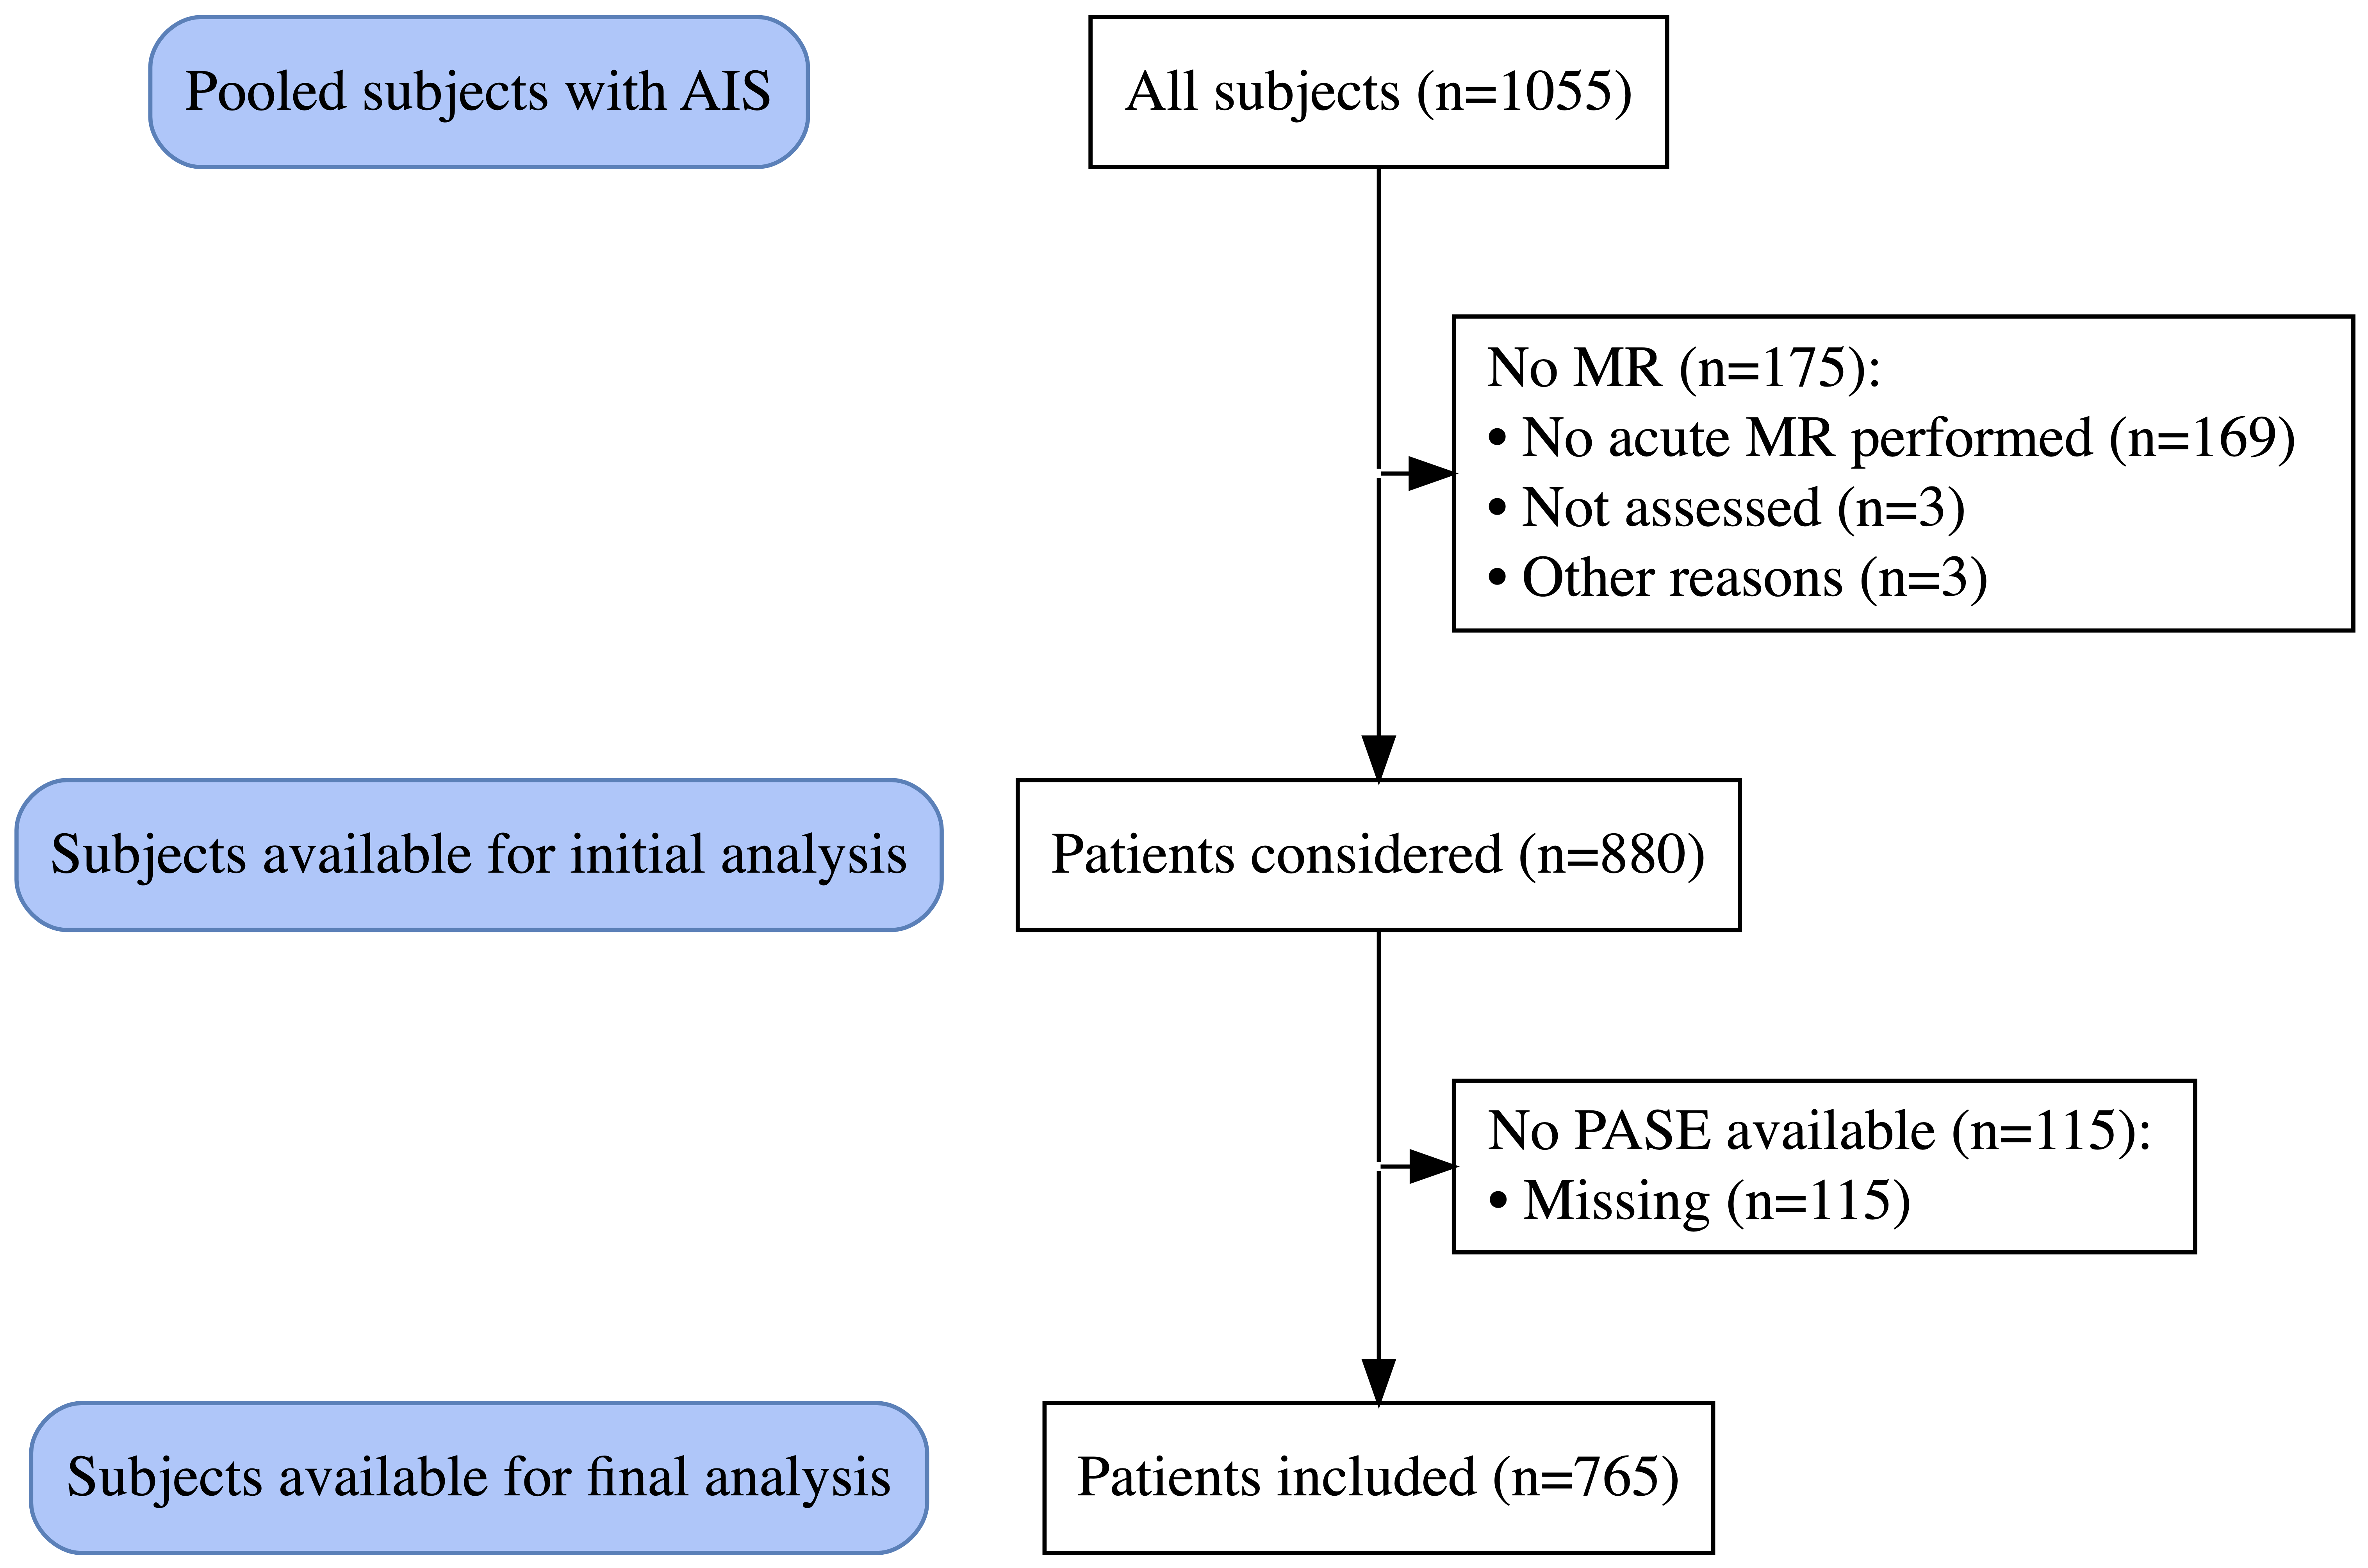
\includegraphics[width=5.5in,height=3.5in]{index_files/figure-latex/dot-figure-2.png}

}

\caption{\label{fig-flowchart}Flowchart of subject included for
analysis}

\end{figure}%

\textsubscript{Source:
\href{https://agdamsbo.github.io/svd-modification/index.qmd.html}{Article
Notebook}}

Baseline characteristics are included with the Table~\ref{tbl-baseline}.

\begin{longtable}[]{@{}
  >{\raggedright\arraybackslash}p{(\columnwidth - 6\tabcolsep) * \real{0.2619}}
  >{\centering\arraybackslash}p{(\columnwidth - 6\tabcolsep) * \real{0.2619}}
  >{\centering\arraybackslash}p{(\columnwidth - 6\tabcolsep) * \real{0.2500}}
  >{\centering\arraybackslash}p{(\columnwidth - 6\tabcolsep) * \real{0.2262}}@{}}

\caption{\label{tbl-baseline}Baseline values SVD burden score}

\tabularnewline

\toprule\noalign{}
\begin{minipage}[b]{\linewidth}\raggedright
\textbf{Characteristic}
\end{minipage} & \begin{minipage}[b]{\linewidth}\centering
\textbf{Overall}, N = 765
\end{minipage} & \begin{minipage}[b]{\linewidth}\centering
\textbf{Female}, N = 280
\end{minipage} & \begin{minipage}[b]{\linewidth}\centering
\textbf{Male}, N = 485
\end{minipage} \\
\midrule\noalign{}
\endhead
\bottomrule\noalign{}
\endlastfoot
SVD score & & & \\
0 & 302 (39\%) & 105 (38\%) & 197 (41\%) \\
1 & 216 (28\%) & 75 (27\%) & 141 (29\%) \\
2 & 142 (19\%) & 61 (22\%) & 81 (17\%) \\
3 & 71 (9.3\%) & 29 (10\%) & 42 (8.7\%) \\
4 & 34 (4.4\%) & 10 (3.6\%) & 24 (4.9\%) \\
Age & 71 (62, 79) & 75 (64, 80) & 70 (61, 77) \\
Admission NIHSS & 4.0 (2.0, 7.0) & 4.0 (2.0, 8.0) & 3.0 (2.0, 7.0) \\
Treated with tPA & 460 (60\%) & 159 (57\%) & 301 (62\%) \\
Treated with EVT & 100 (13\%) & 30 (11\%) & 70 (14\%) \\
Pre-stroke PASE score & 108 (60, 161) & 89 (55, 136) & 116 (71, 175) \\
Living alone & 203 (27\%) & 120 (43\%) & 83 (17\%) \\

\end{longtable}

\textsubscript{Source:
\href{https://agdamsbo.github.io/svd-modification/index.qmd.html}{Article
Notebook}}

Scoring reliability between raters has been compared using different
metrics, to show different nuances to the performance, see
Table~\ref{tbl-irr}. The main performance measure is the intraclass
correlation ceofficient.

\begin{longtable}{lrrrrr}

\caption{\label{tbl-irr}Inter rater reliability testing}

\tabularnewline

\toprule
Variable & Agreement & Krippendorffs\_Alpha & Fleiss\_Kappa & Brennan\_Predigers\_Kappa & IntraclCorrCoef \\ 
\midrule\addlinespace[2.5pt]
microbleed & $0.90$ & $0.65$ & $0.65$ & $0.80$ & $0.65$ \\ 
lacunes & $0.83$ & $0.56$ & $0.56$ & $0.66$ & $0.56$ \\ 
wmh & $0.88$ & $0.72$ & $0.72$ & $0.75$ & $0.72$ \\ 
atrophy & $0.81$ & $0.54$ & $0.54$ & $0.63$ & $0.54$ \\ 
score & $0.62$ & $0.46$ & $0.46$ & $0.52$ & $0.75$ \\ 
\bottomrule

\end{longtable}

\textsubscript{Source:
\href{https://agdamsbo.github.io/svd-modification/index.qmd.html}{Article
Notebook}}

Below is the initial evaluation of possible PA effect modification on
classical risk factors, Table~\ref{tbl-olr}. These results indicates no
effect modification as odds ratios are largely unchanged, when PA is
introduced in the model (on the right). This may not be the optimal
method for this kind of evaluation, though.

\begin{table}

\caption{\label{tbl-olr}Multivariate, ordianal, logistic regression
analysis without and with PASE score included}

\centering{

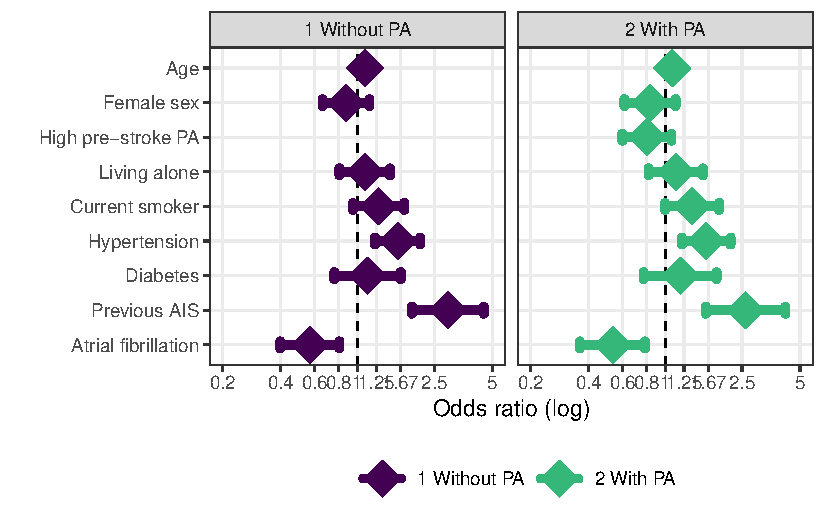
\includegraphics{index_files/figure-pdf/tbl-olr-1.pdf}

}

\end{table}%

\textsubscript{Source:
\href{https://agdamsbo.github.io/svd-modification/index.qmd.html}{Article
Notebook}}

Based on the preliminary SVD-scores, SVD score distribution stratified
by PA quartile is presented in Figure~\ref{fig-svd_dist}.

\phantomsection\label{cell-fig-svd_dist}
\begin{figure}[H]

\centering{

\captionsetup{labelsep=none}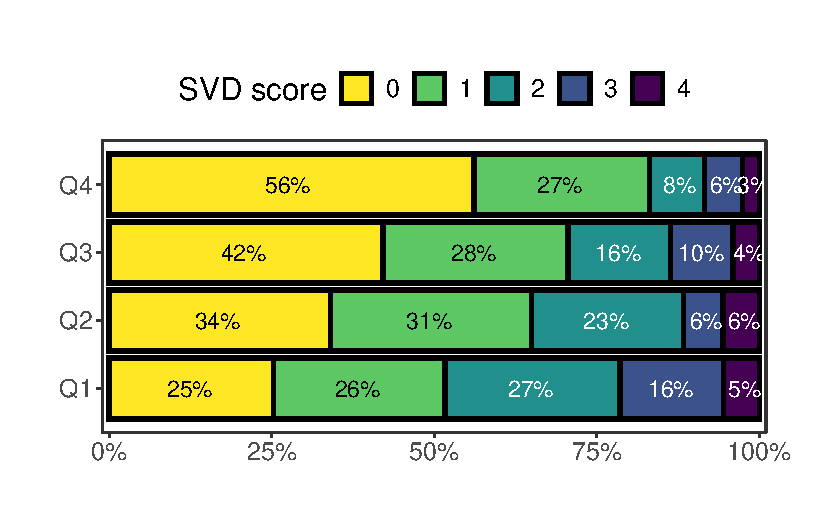
\includegraphics{index_files/figure-pdf/fig-svd_dist-1.pdf}

}

\caption{\label{fig-svd_dist}}

\end{figure}%

\textsubscript{Source:
\href{https://agdamsbo.github.io/svd-modification/index.qmd.html}{Article
Notebook}}

\subsection{Discussion}\label{discussion}

The numbers and figures presented here are very much preliminary and
should only be used for discussion and inspiration. Also, if you have
any interest in collaboration, please reach out!

\phantomsection\label{refs}
\begin{CSLReferences}{1}{0}
\bibitem[\citeproctext]{ref-landman2021}
Landman, Thijs Rj, Dick Hj Thijssen, Anil M. Tuladhar, and Frank-Erik de
Leeuw. 2021. {``Relation between physical activity and cerebral small
vessel disease: A nine-year prospective cohort study.''}
\emph{International Journal of Stroke: Official Journal of the
International Stroke Society} 16 (8): 962--71.
\url{https://doi.org/10.1177/1747493020984090}.

\bibitem[\citeproctext]{ref-moniruzzaman2020}
Moniruzzaman, Mohammad, Aya Kadota, Hiroyoshi Segawa, Keiko Kondo,
Sayuki Torii, Naoko Miyagawa, Akira Fujiyoshi, et al. 2020.
{``Relationship Between Step Counts and Cerebral Small Vessel Disease in
Japanese Men.''} \emph{Stroke} 51 (12): 3584--91.
\url{https://doi.org/10.1161/STROKEAHA.120.030141}.

\bibitem[\citeproctext]{ref-torres2019}
Torres, Elisa R., Siobhan M. Hoscheidt, Barbara B. Bendlin, Vincent A.
Magnotta, Gabriel D. Lancaster, Roger L. Brown, and Sergio Paradiso.
2019. {``Lifetime Physical Activity and White Matter Hyperintensities in
Cognitively-Intact Adults.''} \emph{Nursing Research} 68 (3): 210--17.
\url{https://doi.org/10.1097/NNR.0000000000000341}.

\end{CSLReferences}



\end{document}
